\section{Implementation}
\subsection{Keypad}
\label{sec:KEYPAD}

The most common method of introducing the password of a security box is the keypad. This is due to its ease of use, and its low cost, compared for instance with a dial combination, or a fingerprint scanner.
\medskip

\begin{figure}[H]
    \centering
    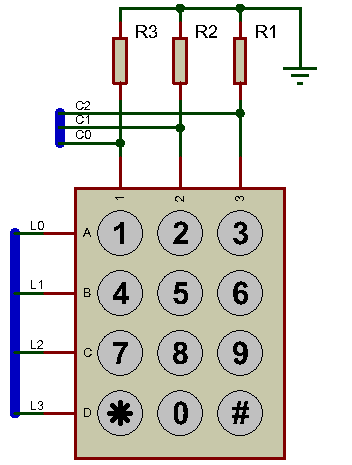
\includegraphics[scale = 0.8]{Graphics/KEYPAD/KEYPAD.PDF}
    \caption{Keypad from Proteus' Libraries}
    \label{fig:KEYPAD}
\end{figure}


In order to implement a keypad in our system, a HIGH level is introduced in one of the line rows and it is constantly circulated among them. When a button is pressed, depending on the column in which a HIGH level is detected and the position of the ‘1’ in the rows, the GAL will be able to show in the output the Binary Coded Decimal (BCD) representation of the number that has been pressed following this fashion:

\begin{table}[H]
    \centering
        \begin{tabular}[t]{lcccc}
            \toprule
            &\textbf{L3..L0}&\textbf{C2...C0}&\textbf{Button}&\textbf{BCD code}\\
            \midrule
                &    0001   & 001     & 1      & 0001     \\
                &    0010   & 001     & 4      & 0100     \\
                &    0100   & 001     & 7      & 0111     \\
                &    1000   & 001     & *      & 1100     \\
                &    0001   & 010     & 2      & 0010     \\
                &    0010   & 010     & 5      & 0101     \\
                &    0100   & 010     & 8      & 1000     \\
                &    1000   & 010     & 0      & 0000     \\
                &    0001   & 100     & 3      & 0011     \\
                &    0010   & 100     & 6      & 0110     \\
                &    0100   & 100     & 9      & 1001     \\
                &    1000   & 100     & \#     & 1111     \\
            \bottomrule
        \end{tabular}
        \caption{Reading to Button Conversion table ~\autocite{SLIDES_5}}
        \label{table: KEYPAD_TABLE}
\end{table}


A ring counter is used in order to rotate the HIGH input bit for the lines. It is a type of counter composed of flip-flops connected together to form a shift register, with the output of the last flip-flop fed to the input of the first, making a "circular" or "ring" structure. In this case, the ring must be initialized with a ‘1’ and after that, the bit will be rotating indefinitely. An example of such counter can be found attached below:

\begin{figure}[H]
    \centering
    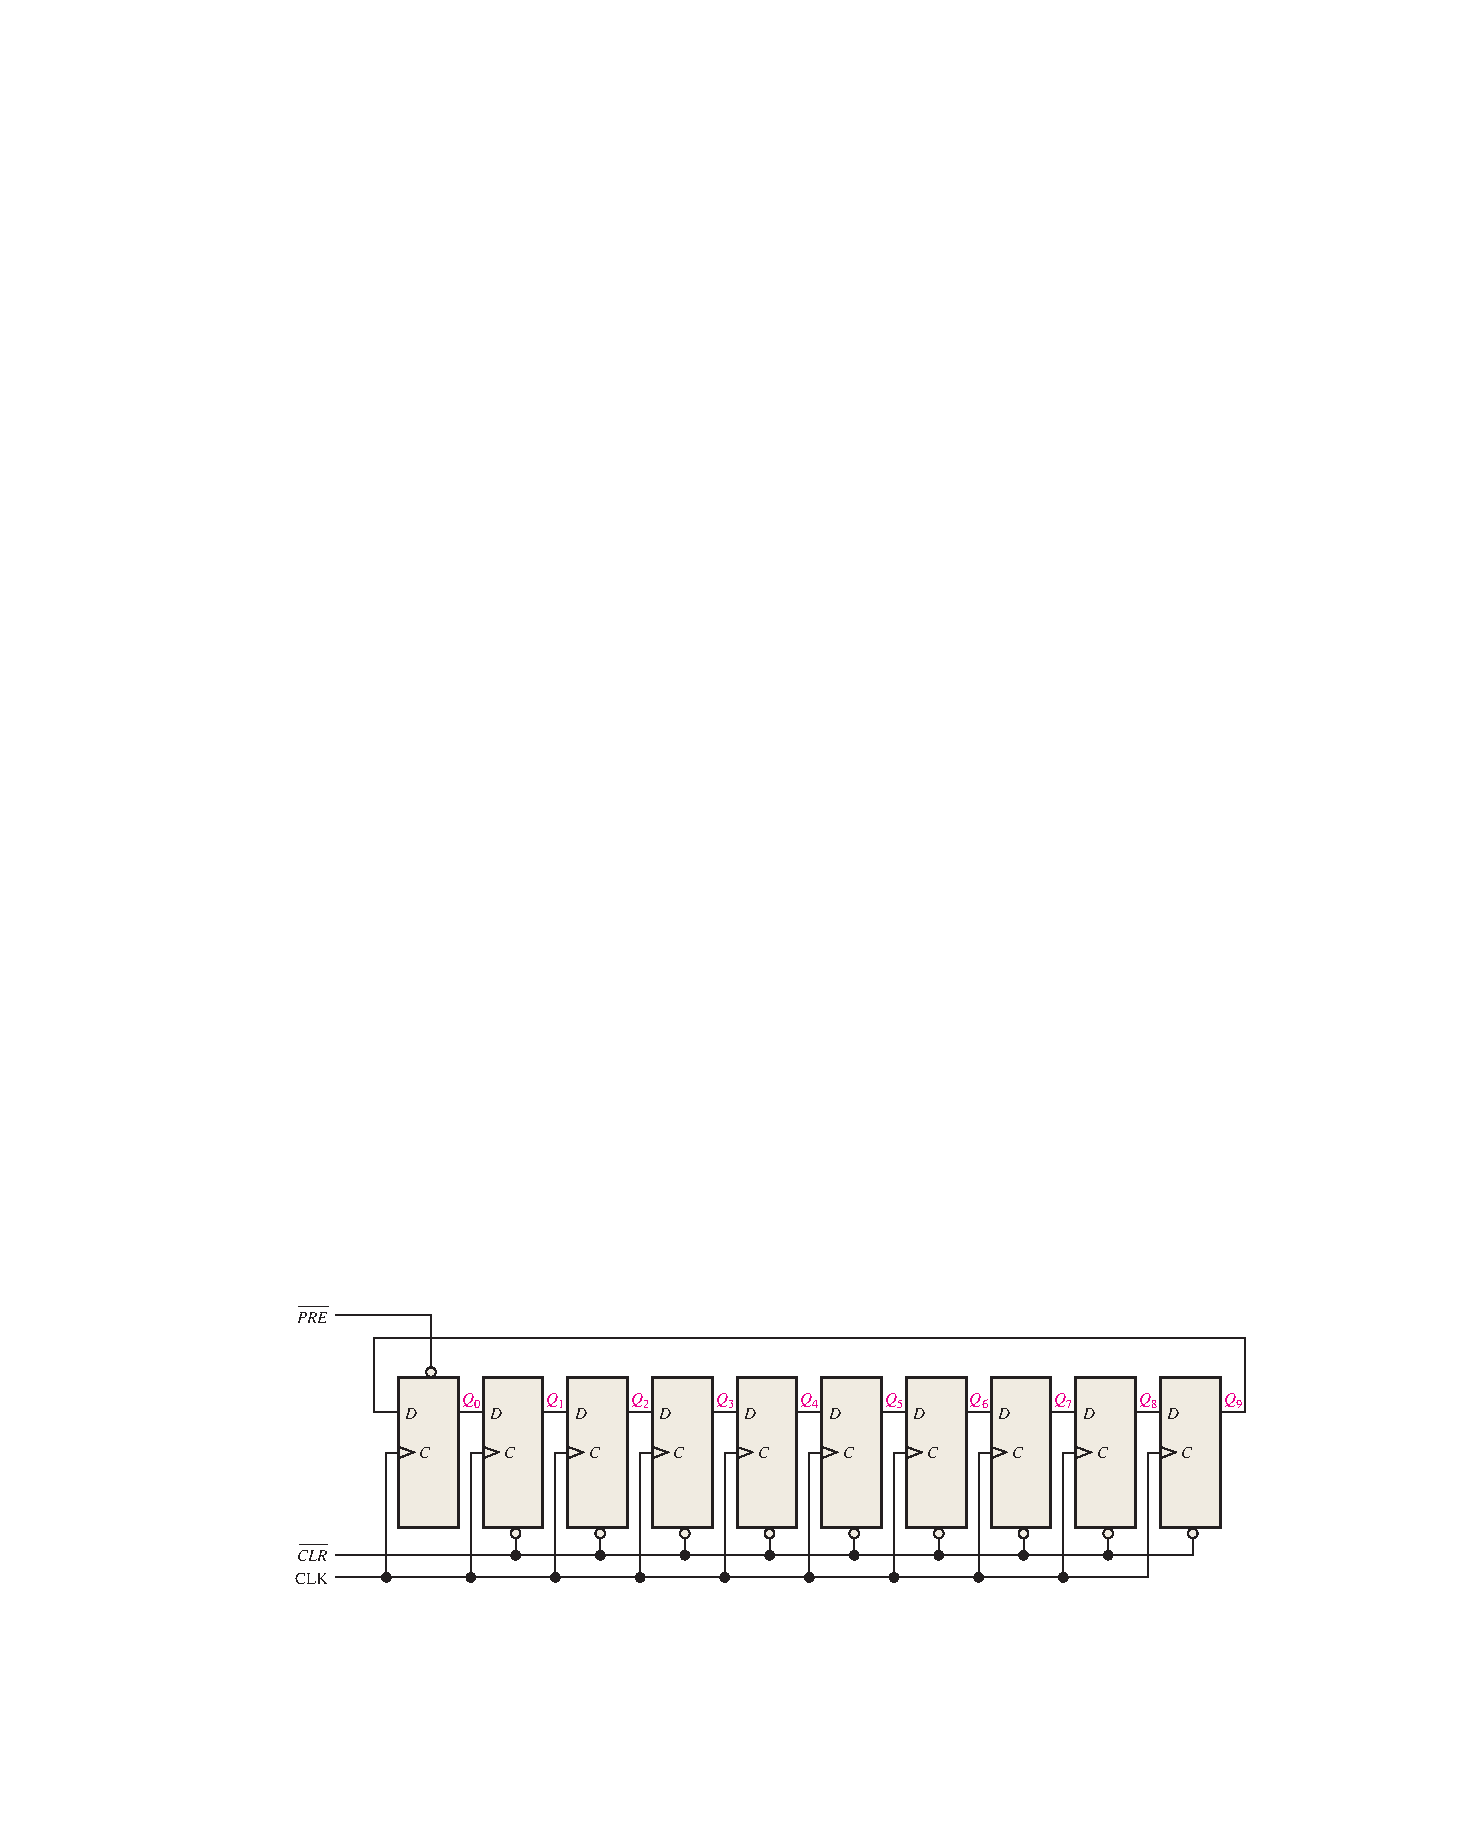
\includegraphics[scale = 0.75]{Graphics/KEYPAD/RING_COUNTER.pdf}
    \caption{10-bit Ring Counter ~\autocite{FLOYD}}
    \label{fig:KEYPAD_RING}
\end{figure}

\medskip
The initialization of the ring counter is done with a pulse coming from the auto start timer that is fed into the \emph{START} input of the GAL, see \textbf{Subsection} \textbf{\ref{sec:ENABLE_AUTOSTART}} for more on this. Once this pulse is detected by the GAL, it introduces a bit in the \emph{l\_temp} internal signal starting the counter. 

\medskip
The \emph{READY} signal is an output that is needed in order to produce the auto start of the system, more on this in \textbf{Subsubsection} \textbf{\ref{sec:AUTOSTART}}.\medskip

Besides, we can also find an output 4 bit array, called \emph{SIG}, which will output the BCD Code that we have previously discussed.\medskip


This I/O configuration can be seen in the following image:\medskip

\begin{figure}[H]
    \centering
    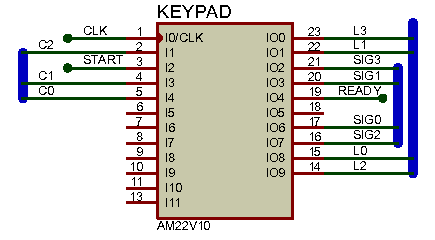
\includegraphics[scale = 1]{Graphics/KEYPAD/KEYPAD_PROTEUS.PDF}
    \caption{Proteus Subassembly of Keypad}
    \label{fig:KEYPAD_PROTEUS}
\end{figure}

\clearpage

The VHDL code that we used for this part of the system is very similar to the one that we used in the practical sessions. It can be found below: 

\vspace{0.5cm}

\inputcode{Code/KEYPAD.vhd}